\chapter{दहन: ईंधन, उत्पाद और ग्रीनहाउस गैसें}\label{ch:g8:combustion-and-fuels}

एक परिवार ऐसे फ़्लैट में सो रहा है जिसके गैस बॉयलर की चिमनी बंद है। \omterm{def:g4:air-a-mixture-of-gases:air}{हवा} न
मिलने से लौ ठीक से नहीं \omterm{def:g4:what-a-fire-needs:burning}{जलती}, और एक अदृश्य, गंधहीन गैस धीरे-धीरे कमरों में
भरती जाती है। रात के दो बजे दीवार पर लगा एक छोटा-सा डिब्बा चीख़ने लगता है:
कार्बन मोनोऑक्साइड अलार्म। सब लोग समय रहते बाहर निकल आते हैं। वही \omterm{def:g4:what-a-fire-needs:fuel}{ईंधन}, ठीक
से \omterm{def:g4:what-a-fire-needs:burning}{जलने} पर, केवल कार्बन डाइऑक्साइड और पानी देता है --- और उस कार्बन
डाइऑक्साइड की अपनी एक कहानी है, जो पूरे ग्रह की \omterm{def:g4:air-a-mixture-of-gases:air}{वायु} में
लिखी है।

\begin{recall}
\omterm{def:g4:what-a-fire-needs:burning}{जलने}, यानी \omterm{def:g4:what-a-fire-needs:burning}{दहन}, के लिए \omterm{def:g4:what-a-fire-needs:fuel}{ईंधन}, ऑक्सीजन और ऊष्मा चाहिए, और इससे नए पदार्थ
बनते हैं (\cref{ch:g4:what-a-fire-needs})। \omterm{def:g4:air-a-mixture-of-gases:air}{वायु} का लगभग पाँचवाँ भाग
ऑक्सीजन है (\cref{ch:g4:air-a-mixture-of-gases})। समीकरण तब संतुलित होता
है जब हर प्रकार का \omterm{def:g7:atoms-and-molecules:atom}{परमाणु} दोनों ओर उतनी ही बार आए
(\cref{ch:g8:balanced-equations})।
\end{recall}

\section{कार्बन और मेथेन का जलना}

\begin{example}[दो दहन]\label{ex:g8:combustion-and-fuels:two}
कार्बन (लकड़ी का कोयला, पत्थर का कोयला) जलकर कार्बन डाइऑक्साइड देता है:
\[
  \ce{C(s) + O2(g) -> CO2(g)}.
\]
मेथेन, प्राकृतिक गैस का मुख्य भाग, जलकर कार्बन डाइऑक्साइड और
पानी देती है:
\[
  \ce{CH4(g) + 2O2(g) -> CO2(g) + 2H2O(l)}.
\]
दोनों में बनी गैस से चूने का पानी दूधिया हो जाता है; मेथेन के साथ ठंडा
गिलास भी धुँधला हो जाता है।
\end{example}

\begin{method}[कार्बन और हाइड्रोजन से बने ईंधन का दहन लिखना]\label{met:g8:combustion-and-fuels:write}
ऐसे \omterm{def:g4:what-a-fire-needs:fuel}{ईंधन} के लिए जिसके \omterm{def:g7:atoms-and-molecules:molecule}{अणुओं} में केवल कार्बन और हाइड्रोजन हों:
\begin{enumerate}
  \item उत्पाद कार्बन डाइऑक्साइड और पानी हैं;
  \item कार्बन को \ce{CO2} से संतुलित करो, फिर हाइड्रोजन को \ce{H2O} से;
  \item दाईं ओर ऑक्सीजन \omterm{def:g7:atoms-and-molecules:atom}{परमाणु} गिनो और उन्हें
        \ce{O2} से संतुलित करो; अगर आधा आ जाए तो सब कुछ दोगुना कर दो।
\end{enumerate}
ब्यूटेन के लिए: \ce{2C4H10 + 13O2 -> 8CO2 + 10H2O}।
\end{method}

\section{पूर्ण और अपूर्ण दहन}

\begin{definition}[पूर्ण और अपूर्ण दहन]\label{def:g8:combustion-and-fuels:complete}
\emph{पूर्ण दहन}\index{पूर्ण दहन} पर्याप्त ऑक्सीजन के साथ होता है:
\omterm{def:g4:what-a-fire-needs:fuel}{ईंधन} का सारा कार्बन कार्बन डाइऑक्साइड बन जाता है।
\emph{अपूर्ण दहन}\index{अपूर्ण दहन} बहुत कम ऑक्सीजन के साथ होता
है: कार्बन का कुछ भाग कार्बन मोनोऑक्साइड,
\ce{CO}, या कालिख बन जाता है, जो कार्बन, \ce{C}, है।
\end{definition}

\begin{example}[ऑक्सीजन की कमी में मेथेन]\label{ex:g8:combustion-and-fuels:incomplete}
बहुत कम \omterm{def:g4:air-a-mixture-of-gases:air}{वायु} होने पर मेथेन जलकर कार्बन मोनोऑक्साइड या कालिख बना सकती है:
\[
  \ce{2CH4 + 3O2 -> 2CO + 4H2O}, \qquad \ce{CH4 + O2 -> C + 2H2O}.
\]
\end{example}

\begin{proposition}[लौ को पढ़ना]\label{prop:g8:combustion-and-fuels:flame}
वायु-छिद्र खुला होने पर बुन्सेन बर्नर \omterm{def:g4:what-a-fire-needs:burning}{जलने} से पहले ही गैस में \omterm{def:g4:air-a-mixture-of-gases:air}{वायु} मिला देता
है: लौ नीली और मुश्किल से दिखने वाली होती है, \omterm{def:g4:what-a-fire-needs:burning}{दहन} पूर्ण होता है।
वायु-छिद्र बंद होने पर गैस को बहुत कम ऑक्सीजन मिलती है: लौ पीली और धुएँदार
होती है, और उसमें पकड़ी गई ठंडी चीज़ को कालिख से काला कर देती है ---
\omterm{def:g4:what-a-fire-needs:burning}{दहन} अपूर्ण है।
\end{proposition}

\begin{omfigure}
\begin{tikzpicture}[font=\small, scale=1.3]
  \pic[transform shape] at (0,0) {bunsen=open};
  \node[anchor=north, align=center] at (0,-0.1) {वायु-छिद्र खुला:\\ नीली लौ, पूर्ण};
  \pic[transform shape] at (4,0) {bunsen=closed};
  \node[anchor=north, align=center] at (4,-0.1) {वायु-छिद्र बंद:\\ पीली लौ, अपूर्ण};
  \draw[<-, omProp, thick] (0.08,0.6) -- (1.4,0.9) node[right, text=black] {वायु-छिद्र};
  \draw[<-, omProp, thick] (-0.4,0.3) -- (-1.3,0.6) node[left, text=black] {गैस};
  \draw[<-, omProp, thick] (4.15,3.3) -- (5.0,3.5) node[right, text=black, align=left]
    {कालिख, कार्बन\\ मोनोऑक्साइड};
\end{tikzpicture}

{\small बुन्सेन बर्नर। नीचे से अंदर आने वाली \omterm{def:g4:air-a-mixture-of-gases:air}{वायु} नीली लौ और \omterm{def:g8:combustion-and-fuels:complete}{पूर्ण दहन}
देती है; उसके बिना लौ पीली और धुएँदार होती है।}
\end{omfigure}

\begin{omfigure}
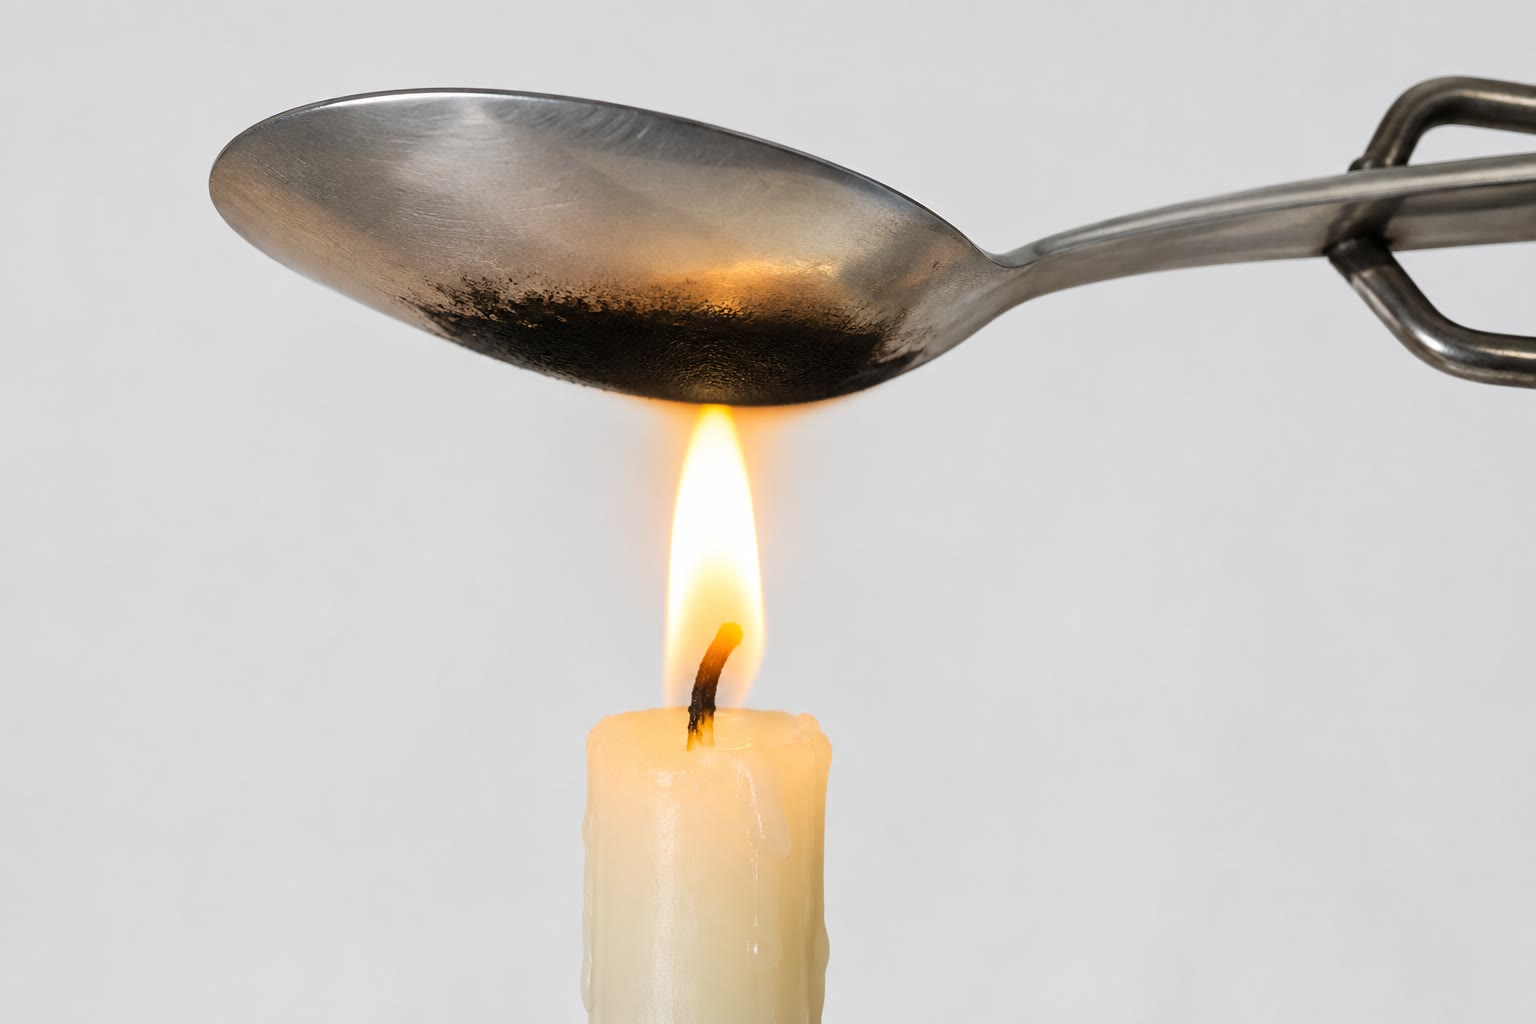
\includegraphics[width=0.45\linewidth]{images/book1/ai/g8-soot-spoon.jpg}

{\small मोमबत्ती की पीली लौ में पकड़ा गया ठंडा चम्मच कालिख से काला हो जाता है:
\omterm{def:g4:what-a-fire-needs:burning}{दहन} अपूर्ण है।}
\end{omfigure}

\section{कार्बन मोनोऑक्साइड, एक ख़ामोश ख़तरा}

\begin{proposition}[कार्बन मोनोऑक्साइड जान क्यों लेती है]\label{prop:g8:combustion-and-fuels:co}
कार्बन मोनोऑक्साइड का न रंग होता है, न गंध, न स्वाद। साँस में जाने पर वह
रक्त में ऑक्सीजन की जगह ले लेती है (कैसे, यह जीवविज्ञान की पुस्तक समझाती है),
जिससे सिरदर्द, नींद आना, और बंद कमरे में बेहोशी और मृत्यु हो जाती है।
यह \omterm{def:g4:air-a-mixture-of-gases:air}{वायु} की कमी में \omterm{def:g4:what-a-fire-needs:burning}{जलने} वाले किसी भी \omterm{def:g4:what-a-fire-needs:fuel}{ईंधन} से बनती है: ठीक से रखरखाव न किया
गया या बंद चिमनी वाला गैस बॉयलर या गीज़र, बंद तंबू में स्टोव, घर के भीतर
इस्तेमाल किया गया बारबेक्यू या जनरेटर।
\end{proposition}

\begin{safety}{\ghs[0.8cm]{GHS02}\ghs[0.8cm]{GHS04}\ghs[0.8cm]{GHS06}\ghs[0.8cm]{GHS08}}
% ledger: ghs:CO
कार्बन मोनोऑक्साइड: अत्यंत ज्वलनशील गैस (GHS02), दाब के साथ भरी
जाती है (GHS04); साँस में लेने पर विषैली (GHS06); बार-बार संपर्क से अंगों
को हानि पहुँचाती है और गर्भस्थ शिशु को नुक़सान पहुँचा सकती है (GHS08)।
\end{safety}

\begin{remark}[विषाक्तता से बचाव]\label{rem:g8:combustion-and-fuels:prevent}
गैस उपकरणों का नियमित रखरखाव किसी पेशेवर से कराया जाता है, चिमनियाँ और
वायु-छिद्र कभी बंद नहीं किए जाते, बारबेक्यू और जनरेटर केवल बाहर
इस्तेमाल होते हैं, और किसी भी बर्नर के पास कार्बन मोनोऑक्साइड अलार्म लगाया जाता है।
\end{remark}

\begin{omfigure}
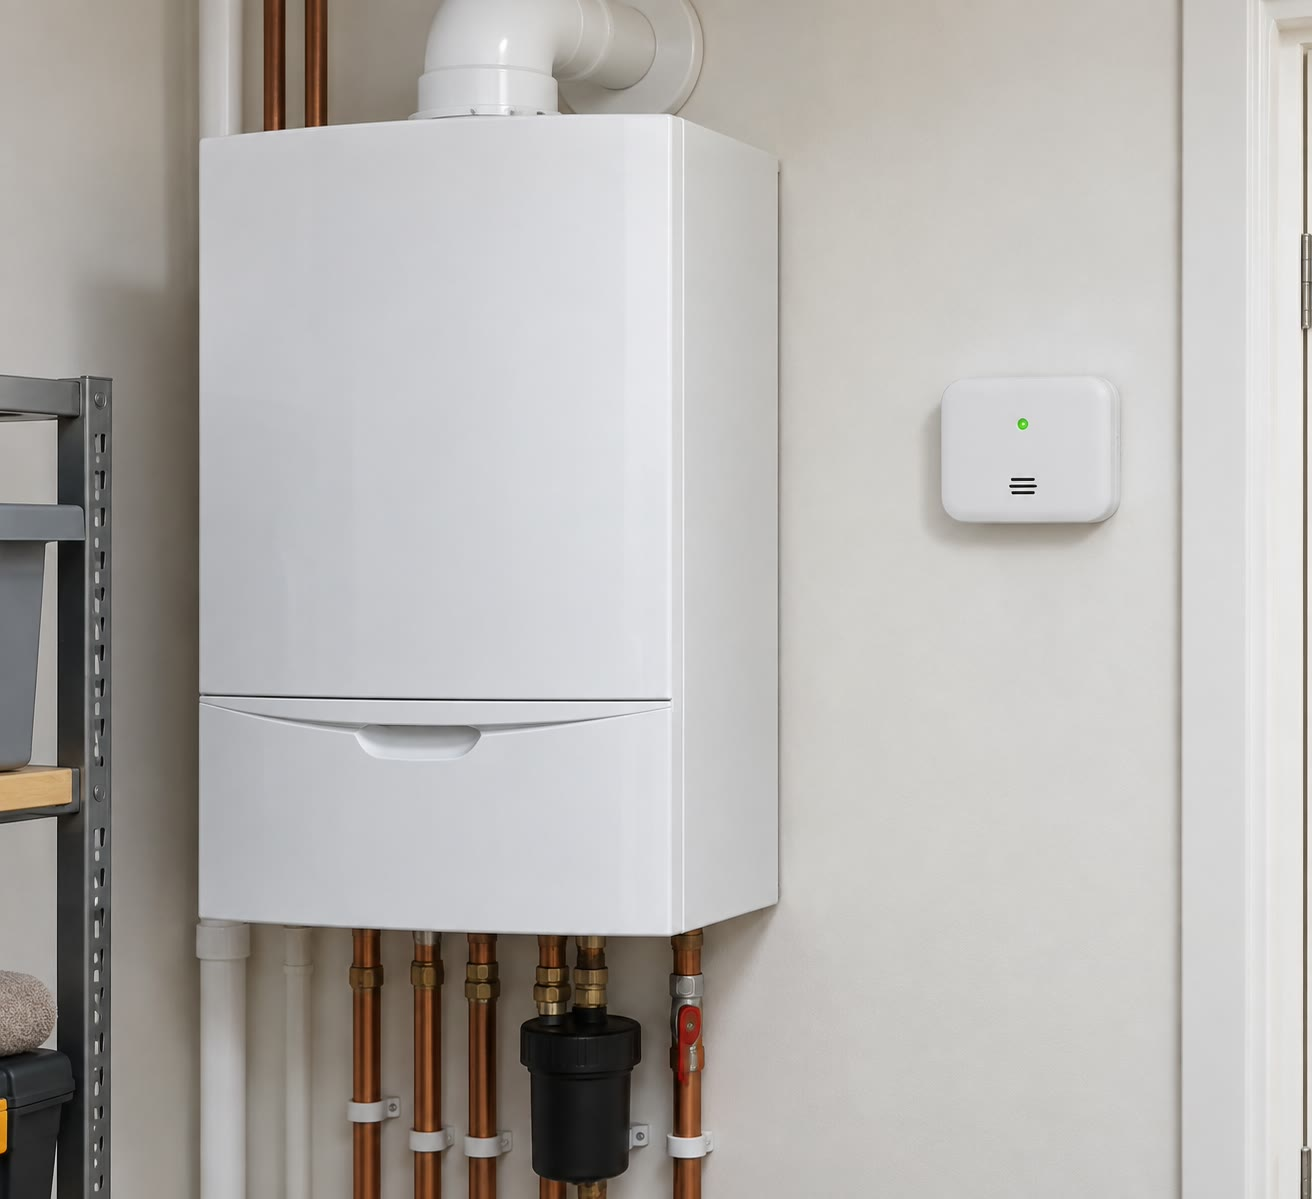
\includegraphics[width=0.45\linewidth]{images/book1/ai/g8-boiler-alarm.jpg}

{\small एक गैस बॉयलर और, उसके बगल में, कार्बन मोनोऑक्साइड अलार्म।}
\end{omfigure}

\section{कार्बन डाइऑक्साइड और ग्रीनहाउस प्रभाव}

\begin{definition}[ग्रीनहाउस गैस]\label{def:g8:combustion-and-fuels:greenhouse}
\emph{ग्रीनहाउस गैस}\index{ग्रीनहाउस गैस} \omterm{def:g4:air-a-mixture-of-gases:air}{वायु} की वह गैस है जो
सूर्य के प्रकाश को आर-पार जाने देती है, पर पृथ्वी की सतह द्वारा अंतरिक्ष की
ओर वापस भेजी गई ऊष्मा का कुछ भाग रोक लेती है, और इस तरह निचले
वायुमंडल को गरम करती है। जलवाष्प, कार्बन डाइऑक्साइड और मेथेन ग्रीनहाउस
गैसें हैं; नाइट्रोजन और ऑक्सीजन नहीं। (ऐसा कैसे होता है, यह भौतिकी की पुस्तक
में समझाया गया है।)
\end{definition}

\begin{proposition}[वायु में कार्बन डाइऑक्साइड बढ़ रही है]\label{prop:g8:combustion-and-fuels:rising}
% ledger: co2:mlo-1959, co2:mlo-2025 (rise 111.4 ppm, +35 %)
\omterm{def:g4:air-a-mixture-of-gases:air}{वायु} में कार्बन डाइऑक्साइड की मात्रा 1959 से प्रशांत महासागर के बीच एक पहाड़
पर बनी वेधशाला में बिना रुके मापी जा रही है। 1959 में यह \omterm{def:g4:air-a-mixture-of-gases:air}{वायु} के दस लाख
भागों में 316 भाग (ppm) थी और 2025 में 427
ppm: एक मनुष्य के जीवनकाल में लगभग \qty{35}{\percent} की वृद्धि,
ज़्यादातर कोयला, तेल और प्राकृतिक गैस \omterm{def:g4:what-a-fire-needs:burning}{जलाने} से। अतिरिक्त कार्बन
डाइऑक्साइड ग्रीनहाउस प्रभाव को बढ़ाती है और जलवायु को गरम करती है।
\end{proposition}

\begin{omfigure}
\begin{tikzpicture}
\begin{axis}[width=0.85\linewidth, height=6cm, xmin=1955, xmax=2030,
    ymin=300, ymax=440, xlabel={वर्ष}, ylabel={कार्बन डाइऑक्साइड (ppm)},
    axis lines*=left, ymajorgrids, grid style={gray!20},
    tick label style={font=\small, /pgf/number format/1000 sep={}},
    label style={font=\small}]
\addplot[omDef, thick, mark=*, mark size=0.8pt]
  table[x=year, y=ppm] {figdata/out/grade-8-co2-record.dat};
\node[anchor=west, font=\small] at (axis cs:1962,306) {1959 में 316 ppm};
\node[anchor=east, font=\small] at (axis cs:2023,428) {2025 में 427 ppm};
\end{axis}
\end{tikzpicture}

{\small \omterm{def:g4:air-a-mixture-of-gases:air}{वायु} में कार्बन डाइऑक्साइड का वार्षिक औसत, 1959 से मापा गया
(NOAA ग्लोबल मॉनिटरिंग लैबोरेटरी के आँकड़े; 1974 से पहले, स्क्रिप्स
इंस्टीट्यूशन ऑफ़ ओशनोग्राफ़ी)।}
\end{omfigure}

\section{जीवाश्म और नवीकरणीय ईंधन}

\begin{definition}[जीवाश्म और नवीकरणीय ईंधन]\label{def:g8:combustion-and-fuels:fossil}
\emph{जीवाश्म ईंधन}\index{जीवाश्म ईंधन} --- कोयला, तेल, प्राकृतिक गैस ---
प्राचीन पौधों और समुद्री जीवों के अवशेषों से लाखों वर्षों में ज़मीन के
नीचे बना। \emph{नवीकरणीय ईंधन}\index{नवीकरणीय ईंधन}
आज उगाए गए पौधों से, या कचरे से, बनता है: लकड़ी, गोबर और खाने के कचरे से
बनी बायोगैस, चुकंदर या गन्ने से बना एथेनॉल।
\end{definition}

\begin{proposition}[कार्बन कहाँ से आता है]\label{prop:g8:combustion-and-fuels:cycle}
पौधे बढ़ने के लिए \omterm{def:g4:air-a-mixture-of-gases:air}{वायु} से कार्बन डाइऑक्साइड लेते हैं। \omterm{def:g8:combustion-and-fuels:fossil}{नवीकरणीय ईंधन} \omterm{def:g4:what-a-fire-needs:burning}{जलाने}
से वह कार्बन डाइऑक्साइड लौटती है जो उसके पौधों ने कुछ साल पहले \omterm{def:g4:air-a-mixture-of-gases:air}{वायु} से ली
थी। \omterm{def:g8:combustion-and-fuels:fossil}{जीवाश्म ईंधन} \omterm{def:g4:what-a-fire-needs:burning}{जलाने} से वह कार्बन मुक्त होता है जो लाखों वर्षों से ज़मीन
के नीचे बंद था: यह \omterm{def:g4:air-a-mixture-of-gases:air}{वायु} में कार्बन डाइऑक्साइड बढ़ाता है।
\end{proposition}

\begin{omfigure}
\begin{tikzpicture}[font=\small,
    box/.style={draw=omDef, fill=omDef!6, rounded corners=2pt, align=center,
      minimum height=0.9cm, text width=2.6cm}]
  \node[box] (air) at (0,3) {वायु में\\ कार्बन डाइऑक्साइड};
  \node[box] (plants) at (5.6,3) {पौधे बढ़ते हैं\\ (\ce{CO2} लेते हैं)};
  \node[box] (fuel) at (5.6,0.4) {लकड़ी, बायोगैस,\\ बायोएथेनॉल};
  \node[box, draw=black!50, fill=black!8] (fossil) at (0,0.4) {कोयला, तेल, गैस:\\ ज़मीन के नीचे};
  \draw[->, thick, omProp] (air) -- (plants);
  \draw[->, thick, omProp] (plants) -- (fuel);
  \draw[->, thick, omProp] (fuel) -- (air);
  \node[text=black, font=\footnotesize, align=left, anchor=north west] at (1.5,1.45)
    {जलना,\\ कुछ साल बाद};
  \draw[->, thick, black!60] (fossil) -- node[midway, left, text=black, font=\footnotesize,
    align=right] {जलना:\\ लाखों वर्षों\\ से जमा\\ कार्बन} (air);
\end{tikzpicture}

{\small \omterm{def:g8:combustion-and-fuels:fossil}{नवीकरणीय ईंधन} \omterm{def:g4:air-a-mixture-of-gases:air}{वायु} को वही कार्बन लौटाते हैं जो उनके पौधों ने उससे लिया
था; \omterm{def:g8:combustion-and-fuels:fossil}{जीवाश्म ईंधन} ज़मीन के नीचे जमा रहा कार्बन जोड़ते हैं।}
\end{omfigure}

\begin{omfigure}
\begin{minipage}[t]{0.48\linewidth}\centering
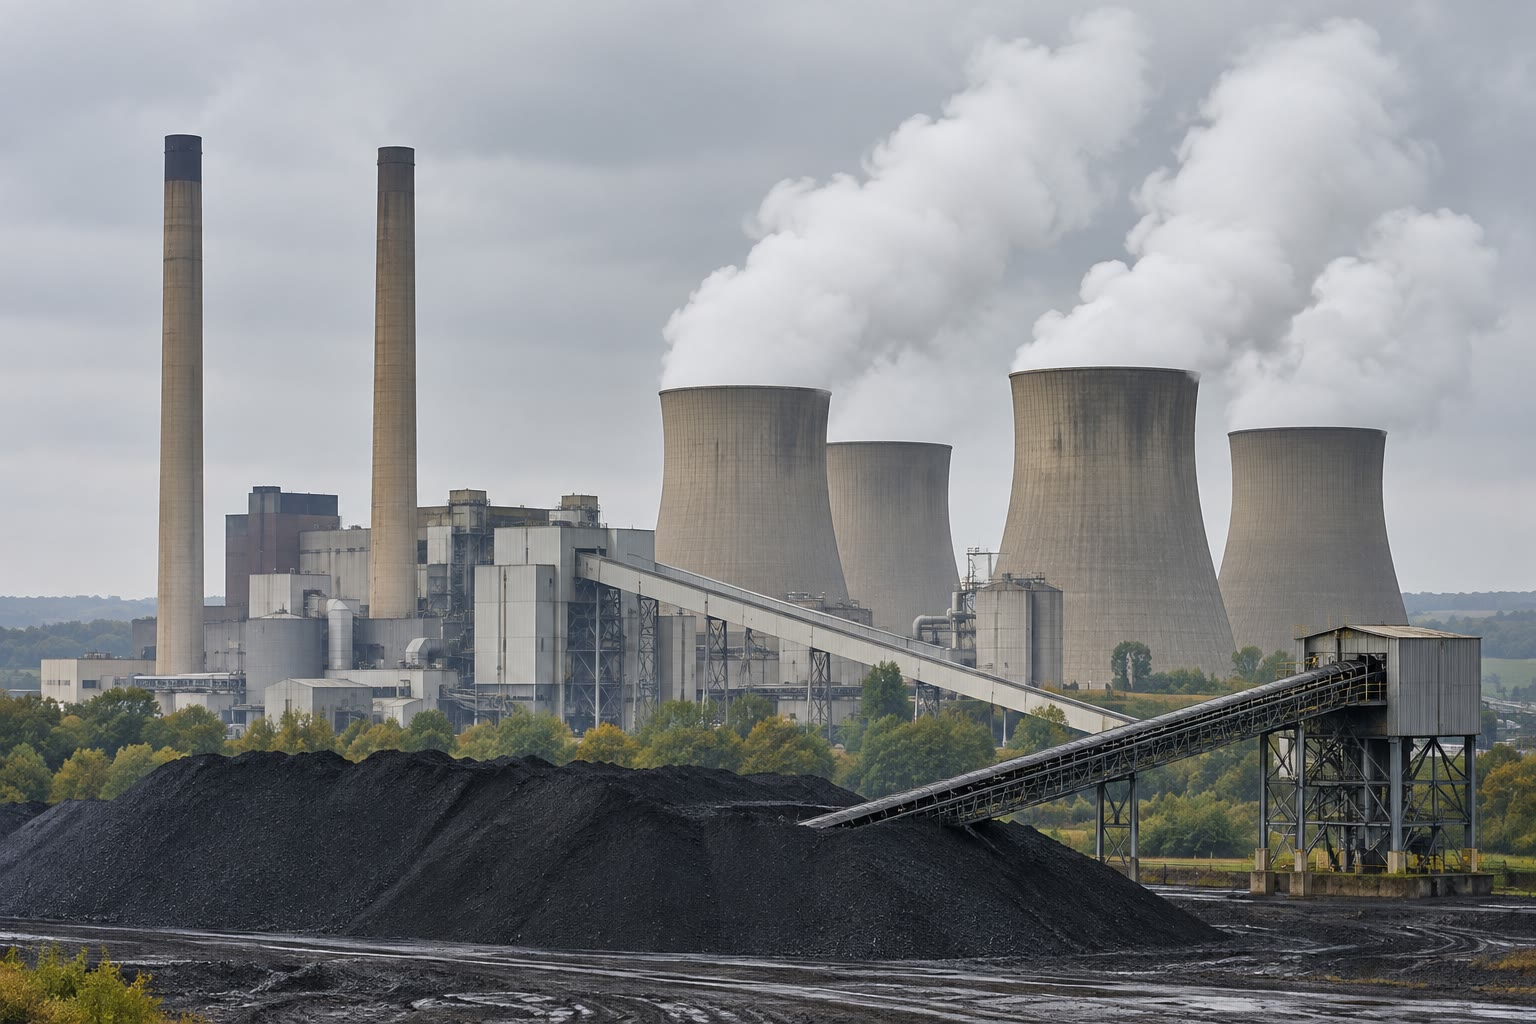
\includegraphics[width=\linewidth,height=4.6cm,keepaspectratio]{images/book1/ai/g8-coal-plant.jpg}

{\small कोयले से चलने वाला बिजलीघर।}
\end{minipage}\hfill
\begin{minipage}[t]{0.48\linewidth}\centering
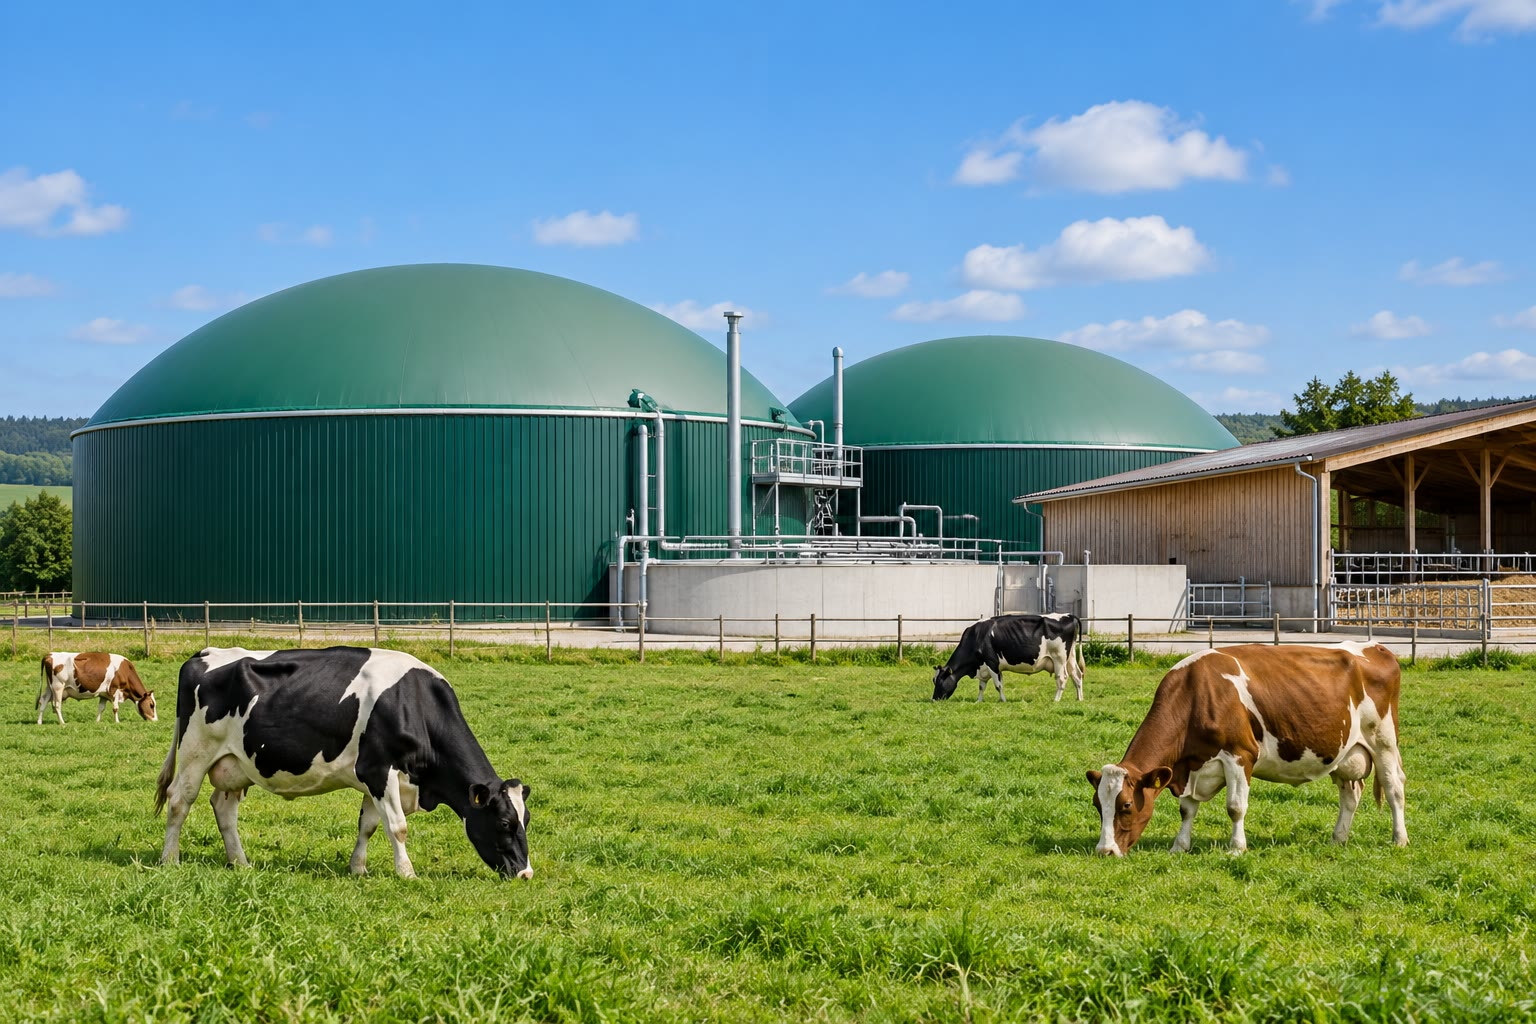
\includegraphics[width=\linewidth,height=4.6cm,keepaspectratio]{images/book1/ai/g8-biogas-farm.jpg}

{\small खेत का बायोगैस संयंत्र: गोबर एक \omterm{def:g8:combustion-and-fuels:fossil}{नवीकरणीय ईंधन} बन जाता है।}
\end{minipage}
\end{omfigure}

\section{अभ्यास}

\begin{exercise}[$\star$]\label{exo:g8:combustion-and-fuels:1}
कार्बन के \omterm{def:g8:combustion-and-fuels:complete}{पूर्ण दहन} का \omterm{def:g8:balanced-equations:equation}{संतुलित समीकरण} लिखो।
\end{exercise}

\begin{exercise}[$\star$]\label{exo:g8:combustion-and-fuels:2}
पूर्ण और \omterm{def:g8:combustion-and-fuels:complete}{अपूर्ण दहन} में क्या अंतर है?
\end{exercise}

\begin{exercise}[$\star$]\label{exo:g8:combustion-and-fuels:3}
कार्बन मोनोऑक्साइड को ख़ामोश ख़तरा क्यों कहा जाता है?
\end{exercise}

\begin{exercise}[$\star$]\label{exo:g8:combustion-and-fuels:4}
जीवाश्म या नवीकरणीय: कोयला, लकड़ी, प्राकृतिक गैस, बायोगैस, पेट्रोल, चुकंदर
से बना एथेनॉल?
\end{exercise}

\begin{exercise}[$\star\star$]\label{exo:g8:combustion-and-fuels:5}
प्रोपेन,
\ce{C3H8}, के \omterm{def:g8:combustion-and-fuels:complete}{पूर्ण दहन} का \omterm{def:g8:balanced-equations:equation}{संतुलित समीकरण} लिखो।
\end{exercise}

\begin{exercise}[$\star\star$]\label{exo:g8:combustion-and-fuels:6}
एथेनॉल, \ce{C2H6O}, ऑक्सीजन में पूरी तरह \omterm{def:g4:what-a-fire-needs:burning}{जलता} है। संतुलित करो:
\ce{C2H6O + O2 -> CO2 + H2O}। % ce-unbalanced-ok (to balance)
\end{exercise}

\begin{exercise}[$\star\star$]\label{exo:g8:combustion-and-fuels:7}
पीली लौ के ऊपर पकड़ी गई कड़ाही नीचे से काली हो जाती है। काला पदार्थ क्या है?
इससे \omterm{def:g4:what-a-fire-needs:burning}{दहन} के बारे में क्या पता चलता है?
\end{exercise}

\begin{exercise}[$\star\star$]\label{exo:g8:combustion-and-fuels:8}
कार्बन डाइऑक्साइड का वक्र पढ़ो: 1980 और 2000 में \omterm{def:g4:air-a-mixture-of-gases:air}{वायु} में लगभग कितनी कार्बन
डाइऑक्साइड थी? उन बीस वर्षों में यह कितने ppm
बढ़ी?
\end{exercise}

\begin{exercise}[$\star\star$]\label{exo:g8:combustion-and-fuels:9}
लकड़ी \omterm{def:g4:what-a-fire-needs:burning}{जलाने} से वर्षों में \omterm{def:g4:air-a-mixture-of-gases:air}{वायु} में कोयला \omterm{def:g4:what-a-fire-needs:burning}{जलाने} की तुलना में कम कार्बन डाइऑक्साइड
क्यों जुड़ती है, हालाँकि दोनों कार्बन डाइऑक्साइड देते हैं?
\end{exercise}

\begin{exercise}[$\star\star$]\label{exo:g8:combustion-and-fuels:10}
कार्बन के कार्बन मोनोऑक्साइड में \omterm{def:g8:combustion-and-fuels:complete}{अपूर्ण दहन} को संतुलित करो:
\ce{C + O2 -> CO}। % ce-unbalanced-ok (to balance)
\end{exercise}

\begin{exercise}[$\star\star\star$]\label{exo:g8:combustion-and-fuels:11}
1959 (316 ppm) से 2025 (427 ppm) तक \omterm{def:g4:air-a-mixture-of-gases:air}{वायु} की कार्बन डाइऑक्साइड कितने
प्रतिशत बढ़ी? निकटतम पूर्ण संख्या तक पूर्णांकित करो।
\end{exercise}

\begin{exercise}[$\star\star\star$]\label{exo:g8:combustion-and-fuels:12}
खिड़की बंद करके एक छोटे कमरे में गैस हीटर चलाया जाता है। इस अध्याय के दो
समीकरणों की मदद से समझाओ कि समय बीतने के साथ \omterm{def:g4:what-a-fire-needs:burning}{दहन} पूर्ण से अपूर्ण कैसे हो
सकता है, और यह ख़तरनाक क्यों है।
\end{exercise}

\section{समस्या: तंबू में स्टोव}

\begin{problem}[{सप्ताहांत समस्या --- एक कैंपिंग स्टोव, उसमें जलने वाली गैस,
उससे क्या बनता है, और वह कभी तंबू के भीतर क्यों नहीं जाता}]
\label{pb:g8:combustion-and-fuels:1}
% ledger: ghs:propane
एक कैंपिंग स्टोव प्रोपेन, \ce{C3H8}, जलाता है, जो एक कारतूस में
\qty{450}{g} भरी है। खुली \omterm{def:g4:air-a-mixture-of-gases:air}{हवा} में लौ नीली होती है। \omterm{def:g8:balanced-equations:equation}{संतुलित समीकरण} से निकाले
गए ये द्रव्यमान-अनुपात लो: \qty{44}{g} प्रोपेन के पूरी तरह \omterm{def:g4:what-a-fire-needs:burning}{जलने} से
\qty{132}{g} कार्बन डाइऑक्साइड बनती है।

\medskip
\noindent\textbf{भाग I --- समीकरण।}
\begin{enumerate}
  \item प्रोपेन के \omterm{def:g8:combustion-and-fuels:complete}{पूर्ण दहन} का \omterm{def:g8:balanced-equations:equation}{संतुलित समीकरण}
        लिखो।
  \item दोनों ओर हर प्रकार के \omterm{def:g7:atoms-and-molecules:atom}{परमाणु} गिनकर इसकी जाँच करो।
  \item \omterm{def:g8:combustion-and-fuels:complete}{अपूर्ण दहन}
        \ce{C3H8 + O2 -> CO + H2O} को संतुलित करो। % ce-unbalanced-ok (to balance)
  \item दोनों में से किसे प्रोपेन के प्रति \omterm{def:g7:atoms-and-molecules:molecule}{अणु} ज़्यादा ऑक्सीजन चाहिए?
\end{enumerate}

\medskip
\noindent\textbf{भाग II --- तंबू के भीतर।}
\begin{enumerate}[resume]
  \item बंद तंबू के भीतर \omterm{def:g4:what-a-fire-needs:burning}{जलाया} गया स्टोव जल्दी ही पीली लौ से \omterm{def:g4:what-a-fire-needs:burning}{जलने} लगता है।
        समझाओ क्यों।
  \item तब कौन-सी ख़तरनाक गैस बनती है? उसके ऐसे दो गुण बताओ
        जिनके कारण उसका पता चलना मुश्किल है।
  \item प्रोपेन के कारतूस पर दो चित्रसंकेत हैं। उनके नाम बताओ और बताओ
        कि हर एक का क्या अर्थ है।
  \item कैंपिंग स्टोव को सुरक्षित रूप से इस्तेमाल करने के दो नियम बताओ।
\end{enumerate}

\medskip
\noindent\textbf{भाग III --- एक कारतूस की कार्बन डाइऑक्साइड।}
\begin{enumerate}[resume]
  \item बनी हुई कार्बन डाइऑक्साइड जली हुई प्रोपेन से कितने गुना भारी
        है?
  \item अतिरिक्त ग्राम कहाँ से आते हैं?
  \item प्रोपेन \omterm{def:g8:combustion-and-fuels:fossil}{जीवाश्म ईंधन} है या \omterm{def:g8:combustion-and-fuels:fossil}{नवीकरणीय ईंधन}? क्या उसे \omterm{def:g4:what-a-fire-needs:burning}{जलाने} से \omterm{def:g4:air-a-mixture-of-gases:air}{वायु} में
        कार्बन डाइऑक्साइड जुड़ती है?
  \item पूरे \qty{450}{g} के कारतूस के पूरी तरह \omterm{def:g4:what-a-fire-needs:burning}{जलने} पर मुक्त होने वाली कार्बन
        डाइऑक्साइड का द्रव्यमान निकालो।
\end{enumerate}
\end{problem}
